
	\documentclass{article}
	\usepackage{amsmath,amssymb}
	\usepackage[inline]{enumitem}
	\usepackage{blindtext}
	\usepackage{booktabs}
	\usepackage{graphicx}
	\usepackage{xcolor}
	\usepackage[vmargin = 1.5in, top = 1in, bottom = 1.2in, letterpaper]{geometry}
	\usepackage{listings}
	\usepackage{courier}
	\usepackage{bm}
	\usepackage{tabu}
	\lstset{
	basicstyle = \small\tt,
	keywordstyle = \tt\color{blue},
	commentstyle = \it\color[cmyk]{1,0,1,0},
	stringstyle = \tt\color[RGB]{128,0,0},
	%frame = single,
	backgroundcolor = \color[RGB]{245,245,244},
	breaklines,
	extendedchars = false,
	xleftmargin = 2em,
	xrightmargin = 2em,
	aboveskip = 1em,
	tabsize = 4,
	showspaces = false
	}
	\begin{document}
	
	% \newfontfamily\courier{Courier New}

	
	\title{STAT 500 Homework 11}
	\author{Yifan Zhu}
	\maketitle
	
	\begin{enumerate}[leftmargin = 0 em, label = \arabic*., font = \bfseries]
	\item
	The choice of the final model is
	\[SalePrice = \beta_1 BasementArea + \beta_2 LivingArea + \beta_3 TotalRoom + \beta_4 Age + \epsilon\]

	From the Backward Elimination, we have
	\begin{center}
		\begin{tabular}{*{3}{p{0.1\textwidth}} *{5}{l}}
	\toprule
Step&Variable Removed&Number Vars In&Partial R-Square&Model R-Square&C(p)&F Value&Pr $>$ F\\
\midrule
1&Garage&4&0.0000&0.7711&4.1794&0.18&0.6719\\
\bottomrule
	\end{tabular}
	\end{center}

	From Stepwise Selection, we have
\begin{center}
	\begin{tabular}{*{6}{p{0.1\textwidth}} *{3}{l}}
	\toprule
Step&Variable Entered&Variable Removed&Number Vars In&Partial R-Square&Model R-Square&C(p)&F Value&Pr $>$ F\\
\midrule
1&LivingArea&&1&0.5514&0.5514&951.805&1225.32&$<.0001$\\
2&BasementArea&&2&0.1522&0.7036&293.249&511.50&$<.0001$\\
3&Age&&3&0.0621&0.7657&25.8848&263.57&$<.0001$\\
4&TotalRoom&&4&0.0055&0.7711&4.1794&23.72&$<.0001$\\
\bottomrule
\end{tabular}
\end{center}

And from all possible models, the final choice have the second largest R-squared value, but have a better $C_p$ than the full model. Thus we still choose this model.



  \item \

\begin{center}
  \begin{tabular}{*{6}{l}}
  \toprule
  Variable&Parameter Estimate&Standard Error&Type II SS&F Value&Pr $>$ F \\
  \midrule
  Intercept&32673&6566.47208&39017274499&24.76&$<.0001$\\
BasementArea&58.12806&3.38917&4.635775E11&294.16&$<.0001$\\
LivingArea&104.75703&4.45529&8.712679E11&552.86&$<.0001$\\
TotalRoom&-6481.53764&1330.68534&37388941590&23.72&$<.0001$\\
Age&-746.48764&46.74967&4.018148E11&254.97&$<.0001$\\
\bottomrule

  \end{tabular}

\end{center}


	\item \

\begin{center}
\begin{tabular}{*{6}{l}}
\toprule
Source&DF&Sum of Squares&Mean Square&F Value&Pr $>$ F\\
\midrule
Model&4&5.277833E12&1.319458E12&837.26&$<.0001$\\
Error&994&1.566478E12&1575933256&&\\
Corrected Total&998&6.844311E12&&&\\
\bottomrule	
\end{tabular}
\end{center}

\item 
The $R^2$ is \textbf{0.7711.}
It means that 77.11\% of the variation in SalePrice of training data can be explained by the multiple linear regression model with BasementArea, LivingArea, TotalArea and Age.


\newpage
\item From the studentizaed residual we can see there are more than 10 outliers whose studentized residual is greater than 3. And there are some potential outliers whose absolute value of studentized residual is greater than 2 but less than 3.

From the leverage plot, we can see that there are more than 10 points whose leverage is greater than 0.0015.

From the Cook'D plot, we can see there are 3 to 4 potential influential points.

\begin{center}
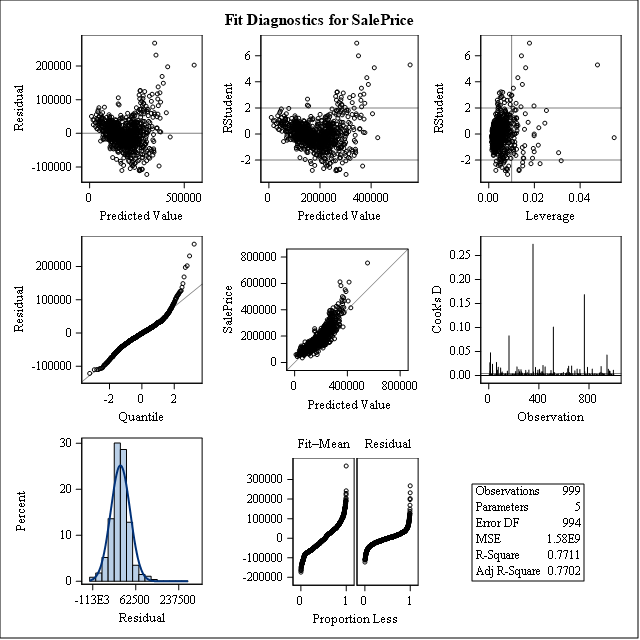
\includegraphics[width = 0.8\textwidth]{fit.png}
\end{center}



\item \ 

\begin{center}
\begin{tabular}{*{6}{l}}
\toprule
Variable&DF&Parameter Estimate&Standard Error&t Value&Pr $> |t|$\\
\midrule
Intercept&1&31813&4520.11936&7.04&$<.0001$\\
BasementArea&1&60.94602&2.46440&24.73&$<.0001$\\
LivingArea&1&98.50489&3.31417&29.72&$<.0001$\\
TotalRoom&1&-5303.86093&986.41063&-5.38&$<.0001$\\
Age&1&-776.22179&31.67872&-24.50&$<.0001$\\
\bottomrule
\end{tabular}
\end{center}


\item \ 

\begin{center}
\begin{tabular}{*{6}{l}}
\toprule
Source&DF&Sum of Squares&Mean Square&F Value&Pr $>$ F\\
\midrule
Model&4&9.037262E12&2.259316E12&1553.51&$<.0001$\\
Error&1919&2.790858E12&1454329388&&\\
Corrected Total&1923&1.182812E13&&	\\	
\bottomrule	
\end{tabular}
\end{center}


\item 
The $R^2$ is \textbf{0.7640.}
It means that 76.40\% of the variation in SalePrice of evaluation data can be explained by the multiple linear regression model with BasementArea, LivingArea, TotalArea and Age.


\item 
$MSE_{evaluation} = 1454329388$ and$ MSE_{training} = 1575933256$. Difference of these two is:
\[ 1575933256 - 1454329388 = 121603868 \]

which is less than $10\%$ of either one.

	


\end{enumerate}

	\end{document}